\section{Learning which targets to reduce together}
\label{sec:batch-policy}
The equation filters reduce work inside a seed region, but the targets grouped in one request also determine that region. A batch can contain targets with high denominator powers and other targets with high numerator rank. Their combined limits can generate equations that neither group needs separately. Dividing the batch can avoid these equations, while repeating preparation and shared algebra can make an unnecessary division slower. We therefore train a model to choose the division from measured complete reduction time. Recent tube-seeding work also uses target groups to control reduction cost~\cite{TubeSeeding2026}; the present method uses ordinary Kira seed regions and the already checked equation filters.

\subsection{Model and integration with Kira}
The model compares five ways to divide a batch: keep all targets together, group equal numerator ranks, group equal extra denominator powers, group equal sectors, or use consecutive groups of at most three targets. A sixth candidate keeps the batch together and disables the equation filter, allowing the new model to avoid an expensive filter or retry. It receives 32 quantities that describe the physical family, the requested powers, and their distribution across the batch. It predicts the complete relative cost of each choice before Kira generates any equations. Each selected group then uses the same fixed seed policy and native row elimination as the preceding method. The existing equation filter acts only when enabled and when the group lies inside its original checked domain. We merge the resulting exact master coefficients after checking that every target has completed.

We compare regression trees, random forests, and extremely randomized forests~\cite{CART1984,Breiman2001Forest,Geurts2006ExtraTrees}. A tree compares the input quantities with learned thresholds and returns predicted costs from the final group of training examples. A forest averages the predictions of several trees. Here each prediction contains six log-cost ratios: the logarithm of a candidate's complete time divided by the time of the undivided batch. Training uses 49 batches, and separate validation uses 49 batches. The candidate with the smallest validation cost is an extremely randomized forest with 32 trees, at most 6 threshold levels, and at least one training example in each final group. Its chosen prediction margin is 0.02 in log-cost units, as defined in Appendix~\ref{app:batch-policy}, and its selected validation costs give 0.7\% less time than fixed partitions. No predictor reaches the required three-percent validation saving, so deployment uses the fixed partitions. The appendix specifies every partition, input, training objective, recovery rule, and physical request, and derives how the independently reduced groups give the complete target reduction.

The training labels include unsuccessful attempts and recovery. Reference construction supplies a common basis and checked coefficients before timing, but the solver receives only the basis and the target definitions. Reference coefficients enter the exact check after reduction. Recorded development, training, and validation reductions take 92.6 minutes, while fitting takes 8.86 seconds; these costs precede deployment and exclude reference construction. The median loading and decision cost in the timed test is 6.73 milliseconds.


Selecting the smallest recorded cost separately for every validation batch would lower the fixed-partition cost by 4.5\%. This comparison uses timing information available only after the calculations and describes the remaining opportunity within these six candidates. It does not describe a deployable predictor. Appendix~\ref{app:batch-policy} defines this retrospective bound.

\subsection{Controls and results}
The reserved comparison uses new rational profiles in the same ten structures at one through four loops, with symbolic dimension. The matched requests contain 1 to 11 targets each. Five repetitions rotate the methods through execution positions on the same worker. The previous method keeps each batch together. One fixed control chooses a partition per graph with the equation filters available; a second fixed control tunes its partitions independently with every ML model disabled. The comparison with the first fixed control measures the added batch-selection application, including its domain checks and loading cost. The second compares the combined workflow with tuned choices that perform no ML inference. All methods share the same exact implementation, basis, worker count, and checks.

Of 108 requests, 96 give matched nontrivial completions. There are 10 failed reference requests, 0 incomplete timed batches, and 2 matched identity-only batches. The comparison record contains 2450 successful results in 2450 calculations, with 90275 exact coefficient comparisons. Every successful result passes its reference check. A total of 34 requested index batches recur in this study's training or validation sets at different rational profiles. The test therefore measures new kinematics and a defined mixture of target batches within known graph structures.


The selected workflow actually calls an equation filter on 4 matched batches. On this subset it uses 7.0\% less time than the separately tuned ML-disabled control. This subset records filter use; its controls can also choose different fixed partitions. Its paired-repetition ratio interval is $[0.834, 1.018]$. This interval includes equal time and does not establish a reliable saving on this subset.


Two cluster allocations reached their time limits before completing all requests. We preserve the 76 complete comparison batches and resume the 22 remaining batches with unchanged models and timing rules. For an interrupted batch, we repeat every method and repetition on one worker. The 4 saved timings from its earlier partial comparison remain available separately and do not enter the ratios. Work assignment uses validation costs only.

Summed batch median time changes from 383.760 seconds for the previous undivided workflow to 389.368 seconds for the selected workflow, giving 1.5\% more time. The fixed control with filters takes 386.251 seconds, and the independently tuned all-ML-disabled control takes 389.826 seconds. Relative to these controls, the selected workflow uses 0.8\% more time and 0.1\% less time, respectively. The selected-to-fixed ratio has a paired-repetition interval of $[0.988, 1.035]$, and the ratio to the all-ML-disabled control has interval $[0.986, 1.025]$. Validation disables the new predictor, so this comparison establishes no additional ML gain from batch selection. Table~\ref{tab:batch-policy} shows the separate graph results, including regressions.


The recorded generation counts sum to 2,429,859 equations for the previous workflow, 2,514,300 for the tuned ML-disabled control, and 2,494,576 for the selected workflow. These are sums of per-batch median counters over reported generation passes, including repeated passes and retries. They describe generated equations rather than the total number of arithmetic operations. Complete time remains the criterion for retaining a model.

\begin{table}[!htbp]\centering\small
\caption{Sum of median complete times in seconds on matched batches. Previous keeps each batch together. Fixed uses one partition per graph with filters. ML off tunes partitions separately with every model disabled. Selected uses the frozen deployment choice.}
\label{tab:batch-policy}
\begin{tabular}{@{}lrrrrr@{}}\toprule
Graph & Batches & Previous & Fixed & ML off & Selected\\\midrule
Three-loop bubble box & 12 & 27.83 & 27.69 & 28.03 & 28.06\\
Four-loop bubble box & 2 & 18.69 & 19.61 & 18.99 & 19.75\\
Planar double box & 12 & 37.29 & 39.87 & 40.36 & 40.05\\
Massive ladder & 12 & 98.23 & 103.36 & 102.32 & 102.17\\
Massless two-point & 10 & 30.38 & 26.66 & 26.76 & 26.56\\
Nonplanar box & 12 & 138.39 & 135.97 & 139.94 & 139.29\\
Virtuality box & 8 & 5.31 & 5.62 & 5.64 & 5.70\\
Pentagon & 8 & 6.20 & 6.07 & 6.12 & 5.99\\
Sunrise & 12 & 13.12 & 12.97 & 12.91 & 13.55\\
Massive vacuum & 8 & 8.31 & 8.41 & 8.76 & 8.23\\
\bottomrule\end{tabular}
\end{table}
\begin{figure}[!htbp]\centering
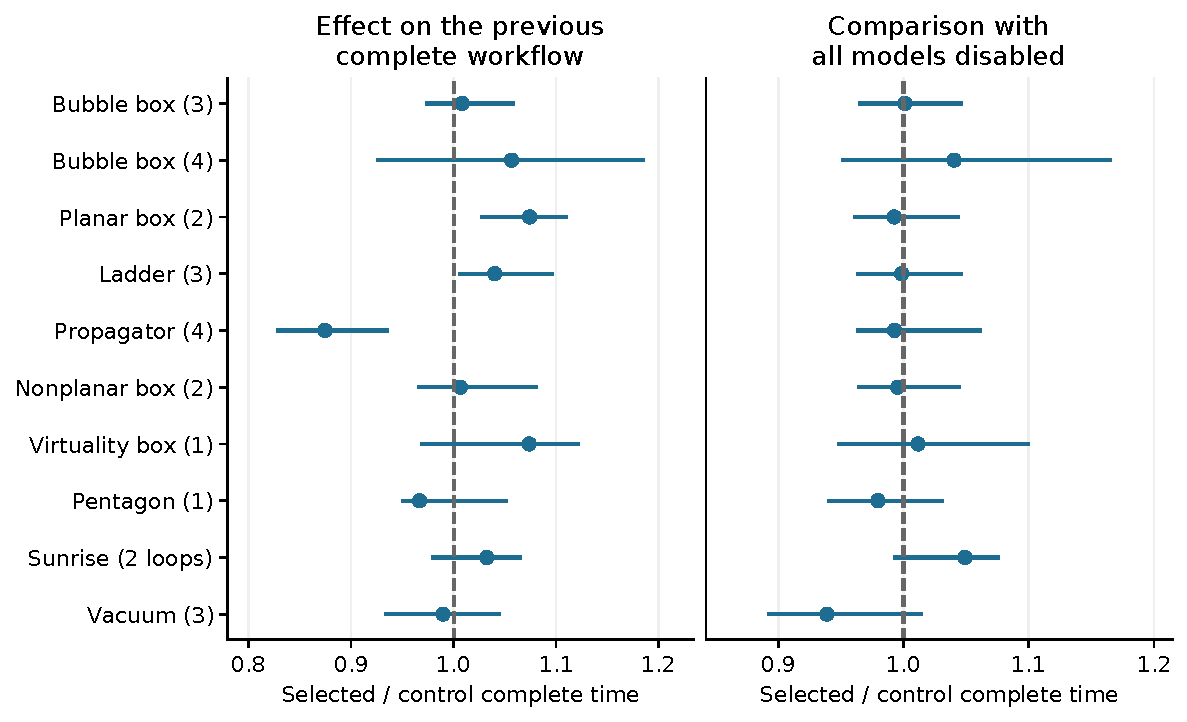
\includegraphics[width=\linewidth]{paper_figures/batch_policy_times.pdf}
\caption{The left panel compares the selected complete workflow with the previous undivided workflow. The right panel compares it with independently tuned fixed partitions with every model disabled. Values below one indicate less time; the dashed line marks equal time. Segments describe paired repetition variation on this workload. Validation disables the new batch predictor; the selected workflow uses the retained fixed partitions and equation-filter settings.}
\label{fig:batch-policy}
\end{figure}
\FloatBarrier

A separate application check starts a new Python process for each request and includes imports, model loading, input and output, and exact checks. Deployment loads only the parts of the frozen policy that it uses: when validation disables the predictor, it retains the fixed choices and domain limits and omits the unused tree arrays. We check that this compact form gives the same choices on every training, validation, and reserved input, without reading reserved timing outcomes. The repeated comparison above retains the original frozen application; this separate check uses the compact form. It completes 36 timed requests over 4 matched batches and gives 1.2\% less time than the previous workflow. These batches are a predeclared subset of the reserved inputs, so this check measures application overhead without adding evidence for new topologies.

The new study extends the batch sizes tested by the earlier equation-filter comparison. It still supplies a master basis and keeps the kinematic invariants rational. General symbolic scattering, arbitrary higher-loop structures, and globally optimal partitions remain outside this evidence. The earlier restricted vacuum recurrence covers its stated one-through-twelve-loop family separately, and its speedup cannot be multiplied by the ratios measured here.
